\documentclass{article}\usepackage[]{graphicx}\usepackage[]{color}
% maxwidth is the original width if it is less than linewidth
% otherwise use linewidth (to make sure the graphics do not exceed the margin)
\makeatletter
\def\maxwidth{ %
  \ifdim\Gin@nat@width>\linewidth
    \linewidth
  \else
    \Gin@nat@width
  \fi
}
\makeatother

\definecolor{fgcolor}{rgb}{0.345, 0.345, 0.345}
\newcommand{\hlnum}[1]{\textcolor[rgb]{0.686,0.059,0.569}{#1}}%
\newcommand{\hlstr}[1]{\textcolor[rgb]{0.192,0.494,0.8}{#1}}%
\newcommand{\hlcom}[1]{\textcolor[rgb]{0.678,0.584,0.686}{\textit{#1}}}%
\newcommand{\hlopt}[1]{\textcolor[rgb]{0,0,0}{#1}}%
\newcommand{\hlstd}[1]{\textcolor[rgb]{0.345,0.345,0.345}{#1}}%
\newcommand{\hlkwa}[1]{\textcolor[rgb]{0.161,0.373,0.58}{\textbf{#1}}}%
\newcommand{\hlkwb}[1]{\textcolor[rgb]{0.69,0.353,0.396}{#1}}%
\newcommand{\hlkwc}[1]{\textcolor[rgb]{0.333,0.667,0.333}{#1}}%
\newcommand{\hlkwd}[1]{\textcolor[rgb]{0.737,0.353,0.396}{\textbf{#1}}}%
\let\hlipl\hlkwb

\usepackage{framed}
\makeatletter
\newenvironment{kframe}{%
 \def\at@end@of@kframe{}%
 \ifinner\ifhmode%
  \def\at@end@of@kframe{\end{minipage}}%
  \begin{minipage}{\columnwidth}%
 \fi\fi%
 \def\FrameCommand##1{\hskip\@totalleftmargin \hskip-\fboxsep
 \colorbox{shadecolor}{##1}\hskip-\fboxsep
     % There is no \\@totalrightmargin, so:
     \hskip-\linewidth \hskip-\@totalleftmargin \hskip\columnwidth}%
 \MakeFramed {\advance\hsize-\width
   \@totalleftmargin\z@ \linewidth\hsize
   \@setminipage}}%
 {\par\unskip\endMakeFramed%
 \at@end@of@kframe}
\makeatother

\definecolor{shadecolor}{rgb}{.97, .97, .97}
\definecolor{messagecolor}{rgb}{0, 0, 0}
\definecolor{warningcolor}{rgb}{1, 0, 1}
\definecolor{errorcolor}{rgb}{1, 0, 0}
\newenvironment{knitrout}{}{} % an empty environment to be redefined in TeX

\usepackage{alltt}

\usepackage{float}

% Set the margins on the page to not be so large
\addtolength{\oddsidemargin}{-.875in}
\addtolength{\evensidemargin}{-.875in}
\addtolength{\textwidth}{1.75in}
\addtolength{\topmargin}{-.875in}
\addtolength{\textheight}{1.75in}

% Take off page numbering
\pagenumbering{gobble}
\IfFileExists{upquote.sty}{\usepackage{upquote}}{}
\begin{document}

\title{%
  2.1.1: R: Simple Linear Regression \\
  \smallskip
  \large Stat 5100: Dr. Bean
}
\date{}

\maketitle

\textbf{Example: } The Toluca Company makes replacement parts for refrigeration equipment.  For a certain part, it takes some time to set up the production process, and then the production of a given lot size can begin.  As part of a cost improvement program, the company wished to better understand the relationship between the lot size (X) and the total work hours (Y).  Data were reported for 25 representative lots of varying size.

\begin{knitrout}
\definecolor{shadecolor}{rgb}{0.969, 0.969, 0.969}\color{fgcolor}\begin{kframe}
\begin{alltt}
\hlkwd{library}\hlstd{(stat5100)}
\hlkwd{data}\hlstd{(toluca)}

\hlcom{# Make a scatterplot of work hours and lotsize}
\hlkwd{plot}\hlstd{(toluca}\hlopt{$}\hlstd{lotsize, toluca}\hlopt{$}\hlstd{workhours)}
\end{alltt}
\end{kframe}
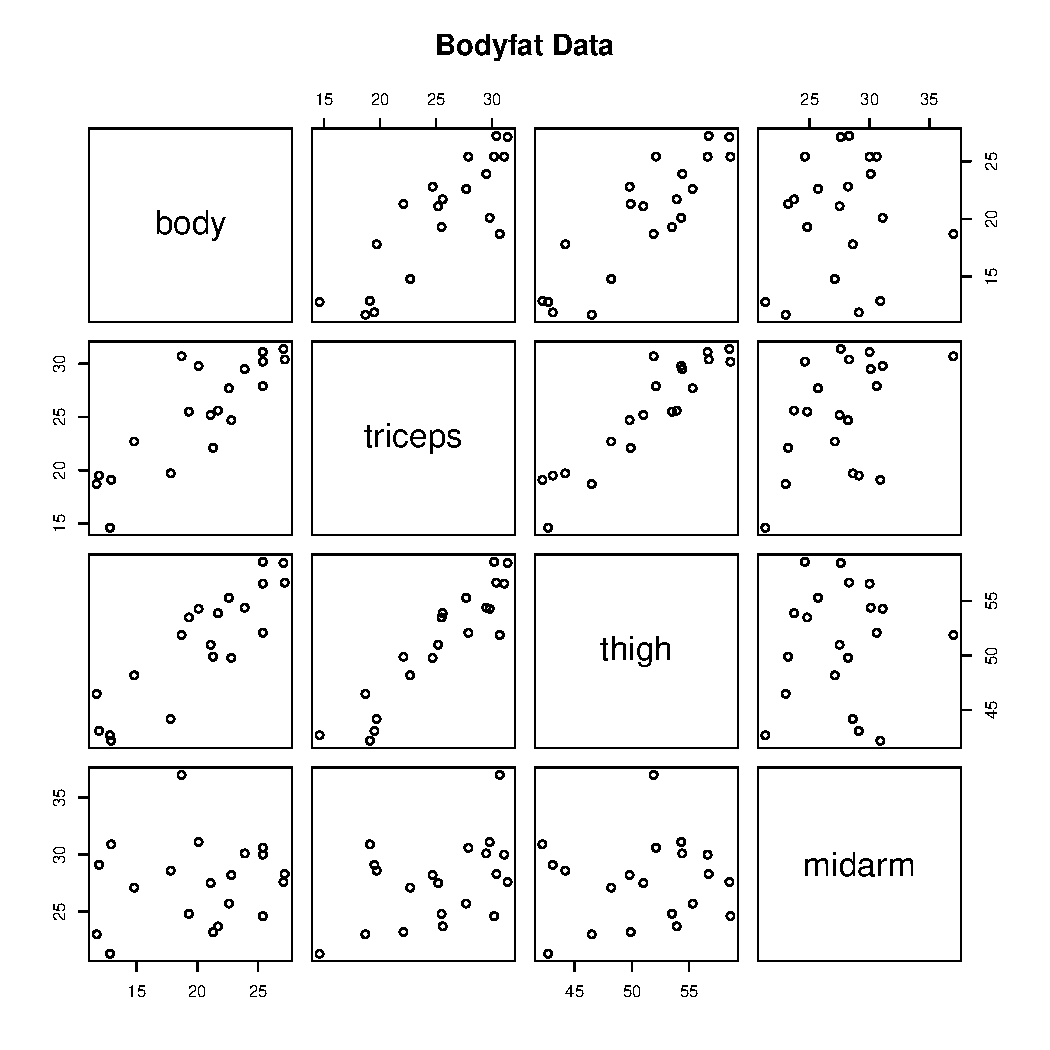
\includegraphics[width=0.6\textwidth]{figure/unnamed-chunk-1-1} 
\begin{kframe}\begin{alltt}
\hlcom{# Give it some labels}
\hlkwd{plot}\hlstd{(toluca}\hlopt{$}\hlstd{lotsize, toluca}\hlopt{$}\hlstd{workhours,}
     \hlkwc{xlab} \hlstd{=} \hlstr{"Lot size"}\hlstd{,} \hlkwc{ylab} \hlstd{=} \hlstr{"Work hours"}\hlstd{,} \hlkwc{main} \hlstd{=} \hlstr{"Toluca Company Data"}\hlstd{,}
     \hlkwc{pch} \hlstd{=} \hlnum{19}\hlstd{)}
\end{alltt}
\end{kframe}
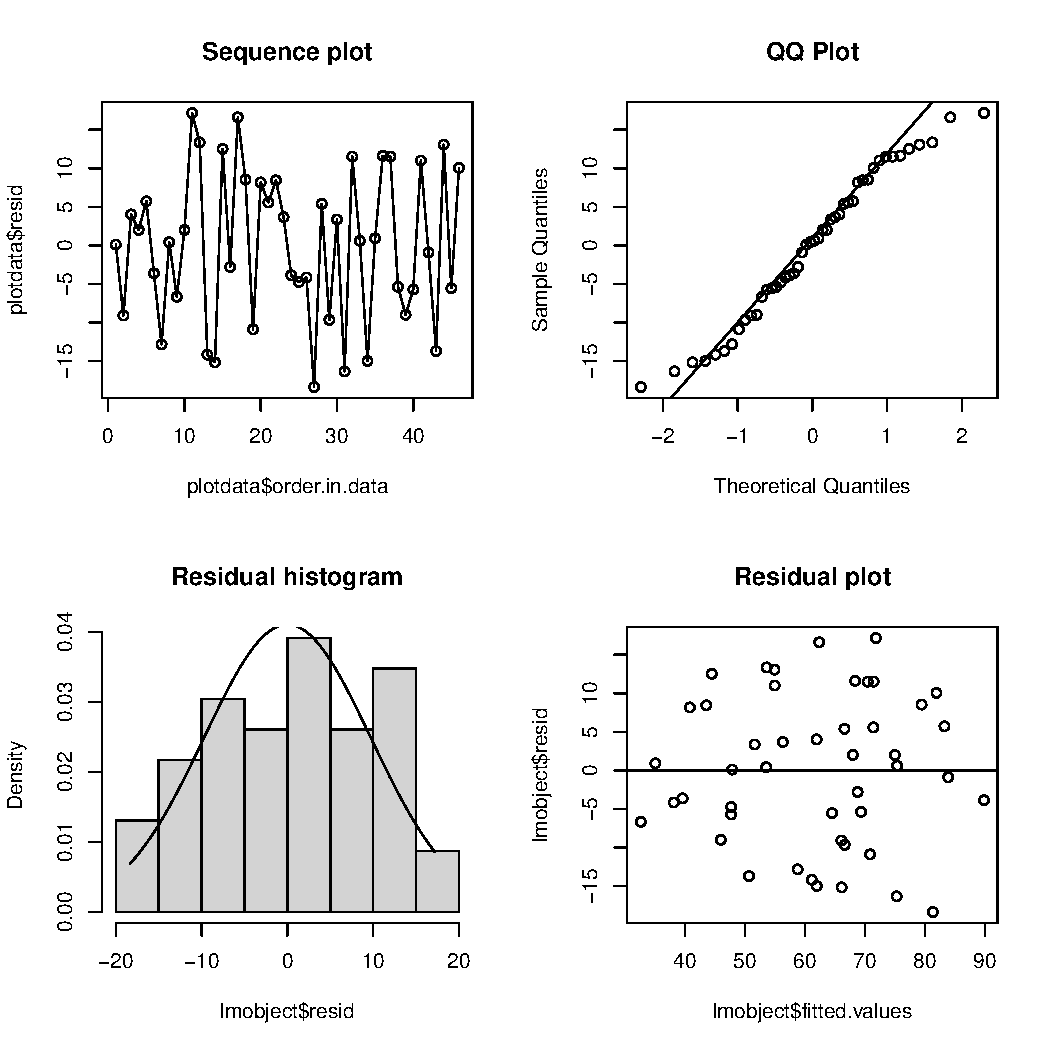
\includegraphics[width=0.6\textwidth]{figure/unnamed-chunk-1-2} 
\begin{kframe}\begin{alltt}
\hlcom{# View some summary and correlation statistics}
\hlkwd{summary}\hlstd{(toluca)}
\end{alltt}
\begin{verbatim}
##     lotsize      workhours    
##  Min.   : 20   Min.   :113.0  
##  1st Qu.: 50   1st Qu.:224.0  
##  Median : 70   Median :342.0  
##  Mean   : 70   Mean   :312.3  
##  3rd Qu.: 90   3rd Qu.:389.0  
##  Max.   :120   Max.   :546.0
\end{verbatim}
\begin{alltt}
\hlkwd{cor}\hlstd{(toluca)}
\end{alltt}
\begin{verbatim}
##             lotsize workhours
## lotsize   1.0000000 0.9063848
## workhours 0.9063848 1.0000000
\end{verbatim}
\begin{alltt}
\hlcom{# Fit a simple linear model with Y = workhours and X = lotsize}
\hlstd{toluca_lm} \hlkwb{<-} \hlkwd{lm}\hlstd{(workhours} \hlopt{~} \hlstd{lotsize,} \hlkwc{data} \hlstd{= toluca)}

\hlcom{# Look at a fit plot for the linear model}
\hlkwd{fit_plot}\hlstd{(toluca_lm,} \hlkwc{main} \hlstd{=} \hlstr{"Fit plot for Toluca Company"}\hlstd{,}
         \hlkwc{xlab} \hlstd{=} \hlstr{"Lot size"}\hlstd{,} \hlkwc{ylab} \hlstd{=} \hlstr{"Work hours"}\hlstd{)}
\end{alltt}
\end{kframe}
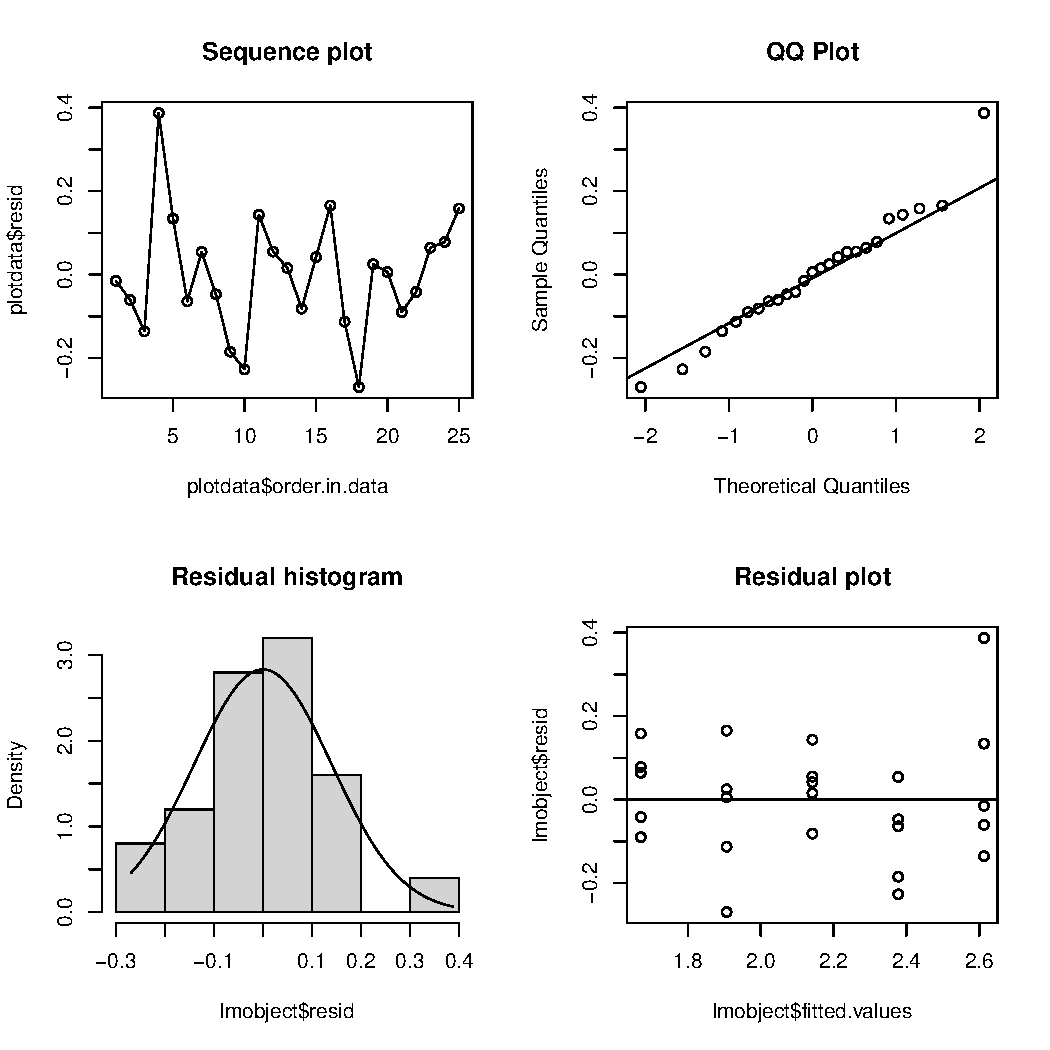
\includegraphics[width=0.6\textwidth]{figure/unnamed-chunk-1-3} 
\begin{kframe}\begin{alltt}
\hlcom{# Look at the ANOVA table and coefficient estimates}
\hlstd{toluca_lm}
\end{alltt}
\begin{verbatim}
## 
## Call:
## lm(formula = workhours ~ lotsize, data = toluca)
## 
## Coefficients:
## (Intercept)      lotsize  
##       62.37         3.57
\end{verbatim}
\begin{alltt}
\hlkwd{anova}\hlstd{(toluca_lm)}
\end{alltt}
\begin{verbatim}
## Analysis of Variance Table
## 
## Response: workhours
##           Df Sum Sq Mean Sq F value    Pr(>F)    
## lotsize    1 252378  252378  105.88 4.449e-10 ***
## Residuals 23  54825    2384                      
## ---
## Signif. codes:  0 '***' 0.001 '**' 0.01 '*' 0.05 '.' 0.1 ' ' 1
\end{verbatim}
\begin{alltt}
\hlcom{# Look at a sample of predicted values}
\hlstd{sample_predicted} \hlkwb{<-} \hlkwd{cbind}\hlstd{(toluca,} \hlkwc{pred_workhours} \hlstd{= toluca_lm}\hlopt{$}\hlstd{fitted.values)}
\hlkwd{head}\hlstd{(sample_predicted)}
\end{alltt}
\begin{verbatim}
##   lotsize workhours pred_workhours
## 1      80       399       347.9820
## 2      30       121       169.4719
## 3      50       221       240.8760
## 4      90       376       383.6840
## 5      70       361       312.2800
## 6      60       224       276.5780
\end{verbatim}
\end{kframe}
\end{knitrout}


\end{document}
